\section{CU5 - Administration du parc de V.M.}

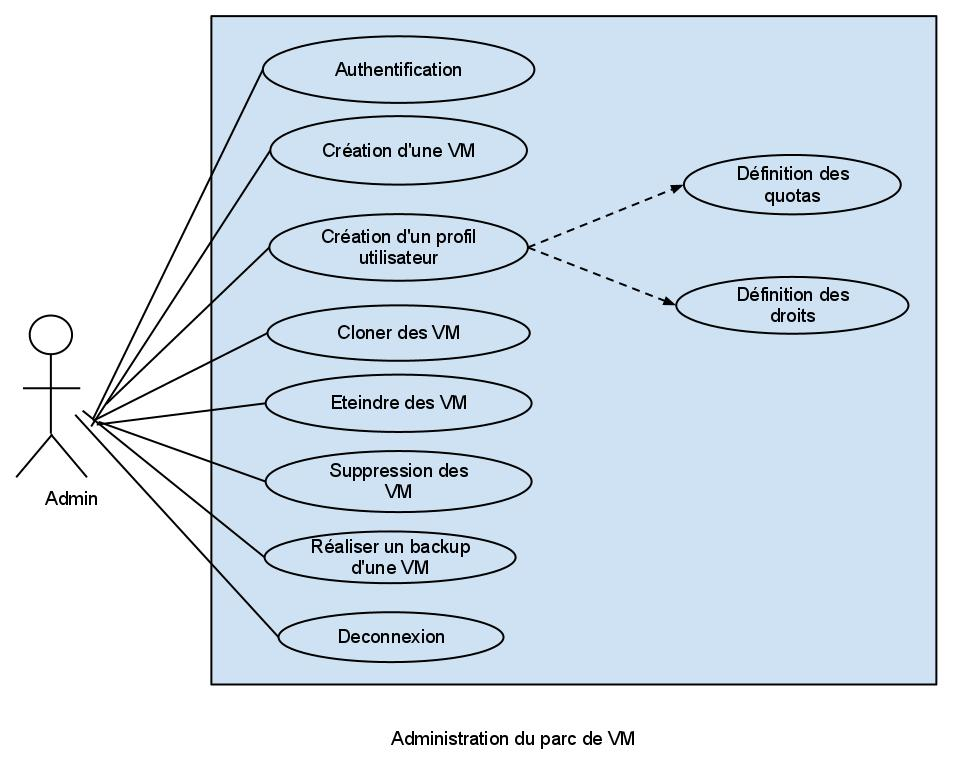
\includegraphics[scale=0.4]{CU5.jpg}

L’administrateur du système devra tout au long de l’année veiller à ce que la plateforme reste exploitable malgré la création/suppression constante de machines virtuelles pour les différents travaux pratique. Sa première tâche sera de créer et mettre à disposition des étudiants ainsi que des enseignants des machines virtuelles de base possédant une configuration minimale laissant les utilisateurs libres de les cloner pour les personnaliser. Il aura également pour rôle de définir les droits d’accès aux différents répertoires de machines virtuelles aux utilisateurs en fonction de leur groupe ou status. 
La sauvegarde de certaines machines sera également dans ses attributions car la perte de certaines machines critiques pourrait grandement pénaliser l’enseignement au département en cas de défaillance du serveur principal.
Il pourra enfin supprimer les machines virtuelles inutiles ou possédée par des utilisateur n’étudiant plus au département.